\documentclass[titlepage]{article}
\usepackage{xcolor} % for different colour comments
\usepackage[left=15mm,right=15mm,top=1in,bottom=1in]{geometry}
\usepackage{framed}
\usepackage{graphicx}
\graphicspath{ {../images/} }
%% Comments
\newif\ifcomments\commentsfalse %i replaced comments true by comment false so the comments will be hidden

\ifcomments
\newcommand{\authornote}[3]{\textcolor{#1}{[#3 ---#2]}}
\newcommand{\todo}[1]{\textcolor{red}{[TODO: #1]}}
\else
\newcommand{\authornote}[3]{}
\newcommand{\todo}[1]{}
\fi

\newcommand{\wss}[1]{\authornote{magenta}{SS}{#1}}
\newcommand{\hm}[1]{\authornote{blue}{HM}{#1}} %Hediyeh
\newcommand{\tz}[1]{\authornote{blue}{TZ}{#1}} %Tahereh
\newcommand{\pl}[1]{\authornote{blue}{PL}{#1}} %Peng


\begin{document}
\title{pylinkvalidator \\
 Design Document Module Guide : newAGEtech, Group H }
\author{Genevieve Okon (Okong), Abraham Omorogbe(Omorogoa),\\
 Eric Le Forte(Leforte)}
\date{\today}
\maketitle


\tableofcontents
\listoffigures
\listoftables

\textbf{Revision History} \\ \normalsize
\pagebreak

\section{Revision History}
\begin{table}[h!]
	\begin{tabular}{| p{5cm} | p{5cm} | p{5cm} |p{5cm} |}    \hline
Revision  &Revision Date &Description of Change &Author\\ \hline
1& 3-11-15& Initiate Design Document&Genevieve Okon\\ \hline
2& 3-11-15& Defined anticipated and likely changes&Genevieve Okon\\ \hline
3& 3-11-15& created Tracability matrix &Abraham Omorogbe\\ \hline
4& 3-11-15& created  Module Hierarchy&Abraham Omorogbe\\ \hline
5& 3-11-15&created pert and Gantt chart&Genevieve Okon\\ \hline
6& 4-11-15& Proofreading and merging of overall content&Genevieve Okon\\ \hline
7& 4-11-15& Use Hierarchy Between Modules&Eric Le Fort\\ \hline
8& 4-11-15&Connection Between Requirements and Design&Eric Le Fort\\ \hline
8& 5-11-15& created Hardware/behaviour Hiding Modules&Abraham Omorogbe\\ \hline
10& 5-11-15& Software Decision Modules&Eric Le Fort\\ \hline
11& 5-11-15& Table of Contents&Genevieve Okon\\ \hline
       \end{tabular}
       
       \caption{Revision History}
       \label{table:Revision History}
\end{table}



\section{Introduction}
The following document details the Module Interface Specifications for the implemented modules in Pylinkvalidator. This will identify and describe the program modules that need to be built in detail so that developers and other viewers can easily understand the program.  Navigation through the program will be simplified for design and maintenance purposes. Complementary documents include the System Requirement Specifications.\\

The rest of the document is organized as follows. Section 3 lists the anticipated and unlikely changes of the software requirements. Section 7 summarizes the module decomposition that was constructed according to the likely changes. Section 4 specifies the connections between the software requirements and the modules. Section 5 will clarify the levels of modules present in the project. Section 6 will compare the design to the requirements provided in the SRS. Section 7 will give a detailed module-by-module breakdown. The rest of the Sections  will trace anticipated changes and modules back to requirements, show the use hierarchy between the modules in the program, set timelines for the rest of the development process and will provide a Gantt and Pert chart to provide a visualization to these task breakdowns.


\section{Anticipated \& Likely Changes}
Anticipated changes are the source of the information that is to be hidden inside the modules. Ideally, changing one of the anticipated changes will only require changing the one module that hides the associated decision.\\

\noindent
AC1: The specific hardware on which the webcrawler is running.\\
AC2: The format of the initial input data.\\
AC3: The format of the input parameters.\\
AC4: The format of the final output data.\\
AC5: The algorithm used for the pylinkvalidator.\\
AC6: The implementation of the html parsers.\\
AC7: How the overall control of the search modules will be made.\\
AC8: The implementation for the visual version of the structure model\\



2.2 Unlikely Changes
The module design should be as general as possible. However, a general system is more complex. Sometimes this complexity is not necessary. Fixing some design decisions at the system architecture stage can simplify the software design. If these decision should later need to be changed, then many parts of the design will potentially need to be modified.
These are few unlikely changes.\\

\noindent
UC1: Input/Output devices (Input: File and/or Keyboard, Output: File, Memory, and/or
Screen)\\
UC2: There will always be a source of input data external to the software.\\
UC3: Output data are displayed to the output device.\\
UC4: Goal of the system is to crawl websites download links and images.\\

\section{Module Hierarchy}
This section contains the module design structure of our project. Modules are summarized in a hierarchy as shown in Table 1. The modules listed below, most of which are leaves in the hierarchy tree, are the modules that will actually be implemented.
\\

\textbf{Modules}\\

\noindent
M1: Option Module\\
M2: Crawler Module\\
M3: HTML Corrector Module\\
M4: Download Resources Module\\
M5: Exact Query Search Module\\
M6: Similar Query Search Module\\
M7: Whitespace Checker Module\\
M8: Find Links Module\\
M9: Check Errors Module\\
M10: Parse Data Module\\
M11: Query Search Module\\
M12: Depth Setter Module\\
M13: Website Structure Modelling Module\\

Note that M5, M6, M7 are submodules of the larger Query Search Module. M2 is the highest level module and utilizes all others internally.\\

\textbf{Hardware hiding}\\

N/A\\

\textbf{Behaviour Hiding Modules}

\begin{itemize}
\item{Download Resources Module}\\
\item{Exact Query Search Module}\\
\item{Similar Query Search Module}\\
\item{Whitespace Checker Module}\\
\item{Find Links Module}\\
\item{Check Errors Module}\\
\item{Parse Data Module}\\
\item{Query Search Module}\\
\item{Website Structure Modelling Module}\\
\end{itemize}

\textbf{Software Decision Modules}

\begin{itemize}
\item{Option Module}\\
\item{Crawler Module}\\
\item{HTML Corrector Module}\\
\item{Depth Setter Module}\\
\end{itemize}



\section{Module Hierarchy Diagram}
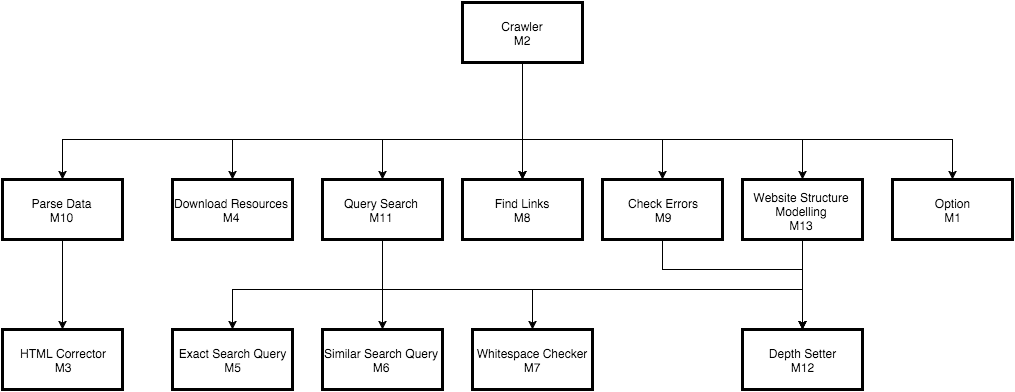
\includegraphics[width=19cm, height=13cm]{UsesDiagram.png}


\section{Connection Between Requirements \& Design}

This design was developed using the requirements document to help guide the decomposition of the project's modules. The requirements were matched to corresponding modules which complete the various tasks. For example, Requirement \#2 from the requirements document (The product shall download resources from a website) will be accomplished using module M4.


\section{Module Decomposition}
\subsection{Hardware Hiding Modules}
N/A
\subsection{Behaviour Hiding Modules}
\subsubsection{Download Resources}
void downloadResources(String: link, String: fileType, String: destination)\\

\textbf{Secrets:}
Parse through the HTML code in the link provided in order to locate all files that match the specified file type. For each file, the result is downloaded into a folder specified by the user.\\

\textbf{Services:}
Writes all resources matching the given file type from the page link to the file specified by destination.\\

\textbf{Implemented By:}
Python

\subsubsection{Exact Query Search}
int[] searchForString(String: query, String: data)\\

\textbf{Secrets:}
Iterates through the data provided and records every instance matching the query String that was passed in. This will be accomplished using the Knuth-Morris-Pratt String searching algorithm.\\

\textbf{Services:}
Returns a list of all occurrences of a given query in the data provided.\\

\textbf{Implemented By:}
Python


\subsubsection{Similar Query Search}
int[] searchForSimilarString(String: query, String: data, int: proximity)\\

\textbf{Secrets:}
Iterates through the data provided and records every instance sufficiently close to matching the query String that was passed in. This will be accomplished using a slight deviation from the Knuth-Morris-Pratt String searching algorithm that recognizes fuzzy string searching.\\

\textbf{Services:}
Returns a list of all occurrences within a certain deviation of a given query in the data provided.\\

\textbf{Implemented By:}
Python

\subsubsection{Whitespace Checker}
boolean isWhitespace(char: character)\\

\textbf{Secrets:}
Checks to see if the character passed in is a tab, a space or a new line character.\\

\textbf{Services:}
Returns whether the character passed in is certain types of whitespace.\\

\textbf{Implemented By:}
Python

\subsubsection{Find Links}
List<Links> findLinks(BeautifulSoup: data, String: destination) Exceptions: No Data Found\\

\textbf{Secrets:}
Parser that parsers through the HTML code in the data provided\\

\textbf{Services:}
Finds all the links ($<$a$>$$<$/a$>$ anchor tags on page) on a page \\

\textbf{Implemented By:}
Python

\subsubsection{Check Errors}
List<Errors> checkErrors(String: link, Array: List of links) Exceptions: Webpage Unavailable\\

\textbf{Secrets:}
Algorithm to check the header in all the links provided \\

\textbf{Services:}
Checks the all the links and reports the error message associated with all the links inputed\\

\textbf{Implemented By:} Python

\subsubsection{Parse Data}
BeautifulSoup parseData(String: link) Exceptions: Invalid Link\\

\textbf{Secrets:}
Converter that converts HTML code link to BeautifulSoup object \\

\textbf{Services:}
Returns Beautiful object for the link given, this will allow modules parse through pages data much faster\\

\textbf{Implemented By:} Python

\subsubsection{Query Search}
void querySearch(String: Query, BeautifulSoup: data, String: choice) Exceptions: Invalid Choice\\

\textbf{Environment Variables:}
rawInput: Users keyboard input\\

\textbf{Secrets:}
An algorithm that figures out what query search type to implement \\

\textbf{Services:}
Writes all resources matching the given file type from the page link to the file specified by destination.\\

\textbf{Implemented By:}
Python

\subsubsection{Website Structure Modelling}
String webStructureModel(String: link, int: depth)\\

\textbf{Secrets:}
 An algorithm that uses the seed link and structures the crawled links by depth\\
 
\textbf{Services:}
It provides a structured model of the website and other site the initial site is connect to. It displays a hierarchy that will show users how crawled link interact with each other.\\

\textbf{Implemented By:}
Python

\subsection{Software Decision Modules}
\subsubsection{Options}
void chooseOption()\\

\textbf{Secrets:}
Obtains input from the user to decide whether they would like to download resources, crawl a website, search for a certain String or model a website. Uses searchDepth to allow the user to set their search depth for all but the download resources option as well as allowing the user to set their seed link.\\

\textbf{Services:}
Gets user input to set various program options related to how the user would like to handle crawling a webpage.\\

\textbf{Implemented By:}
Python

\subsubsection{Crawler}
void crawler()\\

\textbf{Secrets:}
Directly calls the methods shown in the Use Hierarchy (found in section 7 of this document) and consolidates the results.

\textbf{Services:}
Delegates various tasks of crawling a webpage to the other methods of this program.\\

\textbf{Implemented By:}
Python

\subsubsection{HTML Corrector}
String HTMLCorrector(String: link)\\

\textbf{Secrets:}
Tries to fix the given String in various ways in order to create a functioning link. This can include fixing the prefix (http://), adding www., or appending the link to the current page's path.\\

\textbf{Services:}
Fixes the link passed in such that it becomes either a functioning link or is flagged as a broken link.\\

\textbf{Implemented By:}
Python

\subsubsection{Depth Setter}
int depthSetter(int depth) Exception: Not positive int\\

\textbf{Environment Variables}\\
rawInput: Users keyboard input\\

\textbf{Secrets:}
Assignor which sets the depth variable\\

\textbf{Services:}
Sets the default max depth variable for the web crawler\\

\textbf{Implemented By:}
Python

\section{Traceability Matrix}
\begin{table}[h!]
\centering
    \begin{tabular}{| p{5cm} | p{5cm} |}    \hline
    Requirements &Modules\\ \hline
    
      R1  &M1, M2, M3, M9, M10 \\ \hline
      R2  &M1, M2, M3, M4, M10 \\ \hline
      R3  &M12 \\ \hline
      R4  &M2 \\ \hline
      R5  &M1, M2, M3, M4, M5, M6, M7, M8, M9, M10, M11, M12, M13 \\ \hline
      R6  &M1, M2, M3, M8, M10, M12, M13 \\ \hline
      R7  &M1, M2, M3, M5, M6, M7, M8, M10, M11, M12 \\ \hline
      
    \end{tabular}
    \caption{Traceback to Requirements}
\label{table:Traceback to Requirements}
\end{table}

\begin{table}[h!]
\centering
    \begin{tabular}{| p{5cm} | p{5cm} |}    \hline
    Requirements &Modules\\ \hline
    
      AC1  & N/A\\ \hline
      AC2  & \\ \hline
      AC3  & R3, R4\\ \hline
      AC4  & \\ \hline
      AC5  & \\ \hline
      AC6  & \\ \hline
      AC7  & \\ \hline
      AC8  & \\ \hline
      
    \end{tabular}
    \caption{Traceback to Anticipated Changes}
\label{table:Traceback to Anticipated Changes}
\end{table}


\section{Use Hierarchy Between Modules}
The figure below depicts the uses relationships between all the modules in the project. It can be seen that the graph is a directed acyclic graph (DAG). The facade design pattern is being used to design this system. Higher level modules in relation to the hierarchy are inherently simpler because they delegate work to  modules from the lower levels.\\

\begin{figure}
	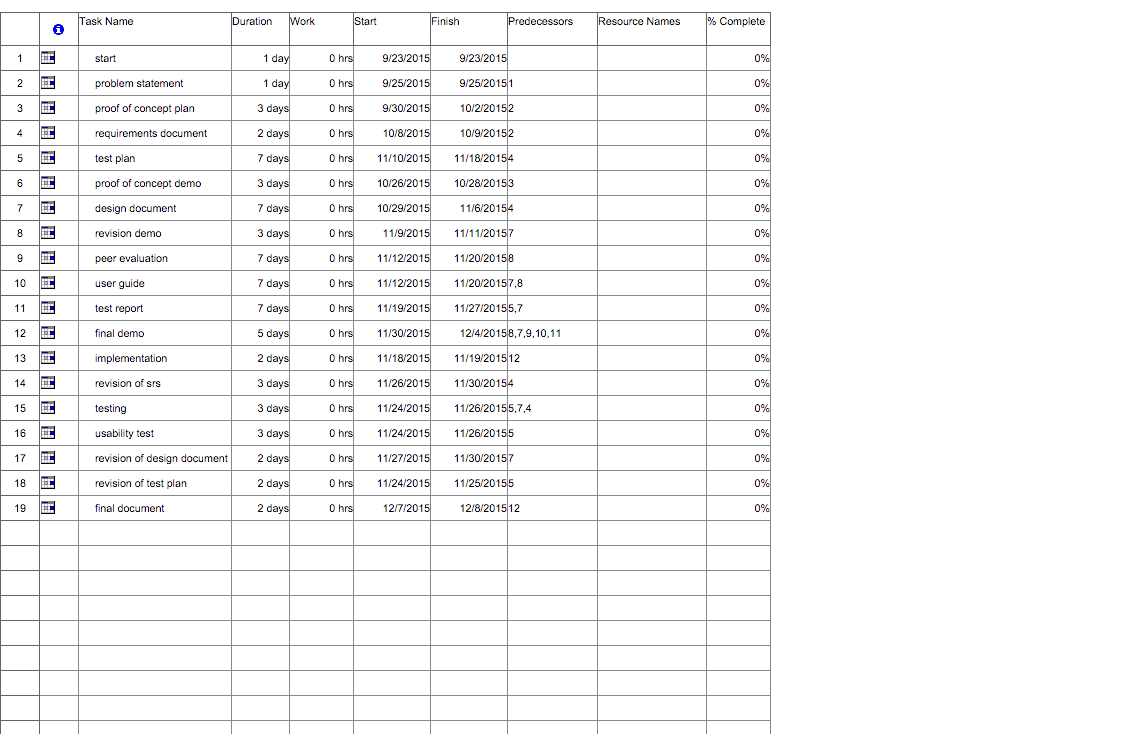
\includegraphics[width=25cm, height=20cm]{detaildesign}
	\caption{Detail Design for the Development Process}
	\label{fig:Detail Design for the Development Process}
\end{figure}


\begin{figure}
	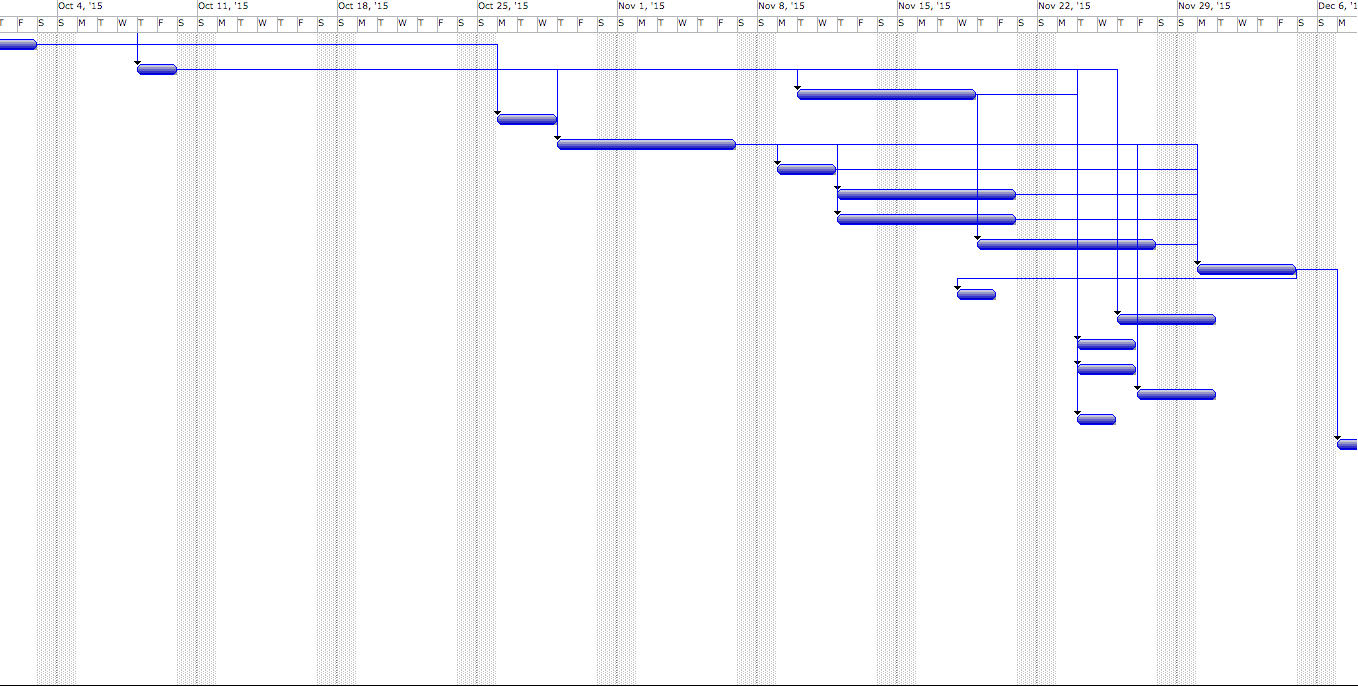
\includegraphics[width=19cm, height=13cm]{gantt}
	\caption{Gantt Chart}
	\label{fig:Gantt}
\end{figure}

\begin{figure}
	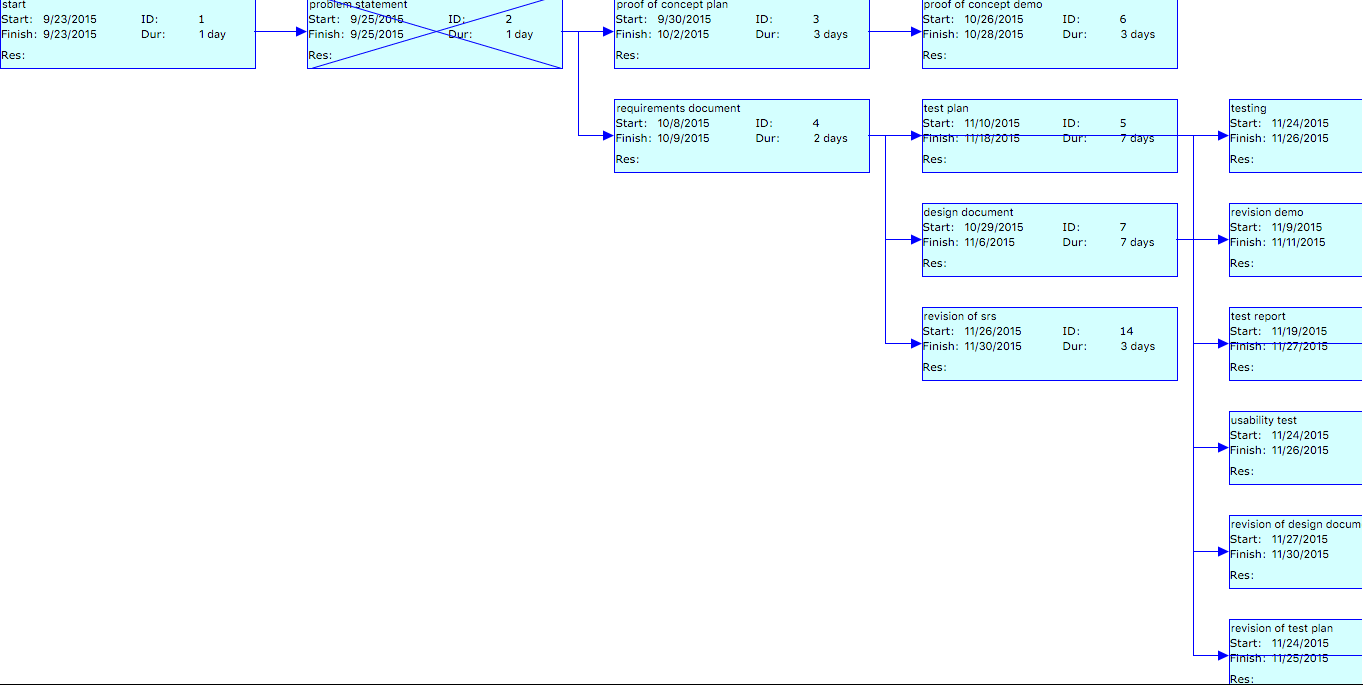
\includegraphics[width=20cm, height=15cm]{pert1}
	\caption{Pert Chart(1)}
	\label{fig:Pert Chart(1)}
\end{figure}

\begin{figure}
	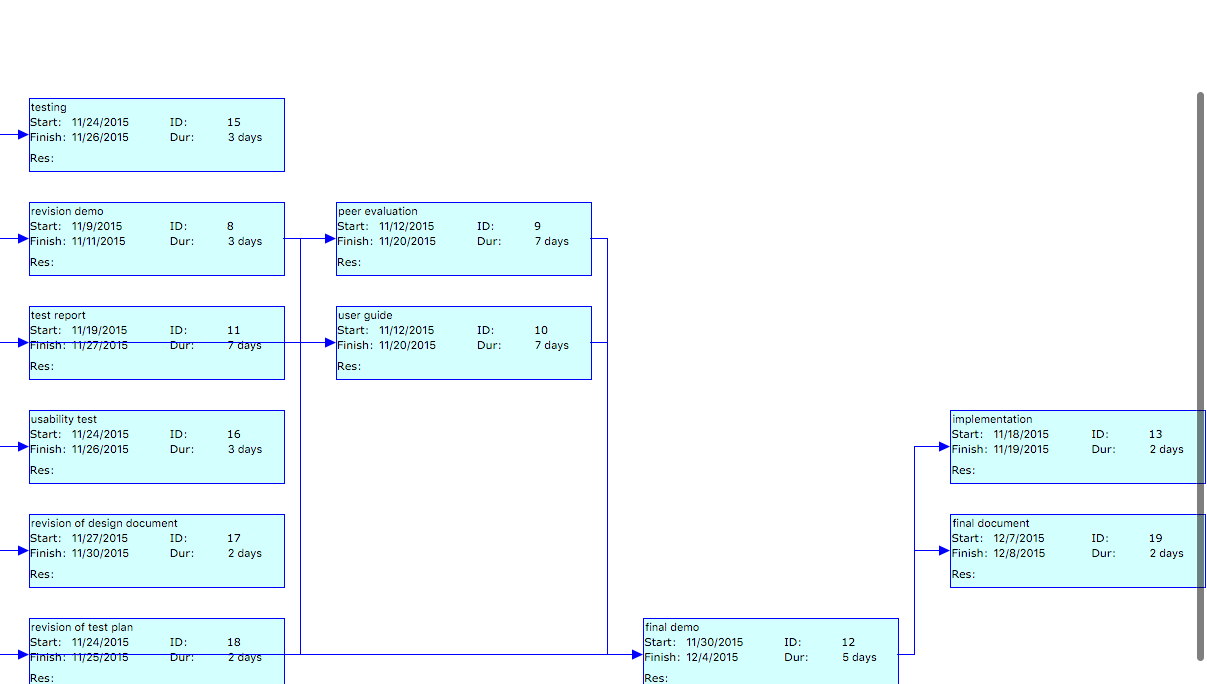
\includegraphics[width=20cm, height=15cm]{pert2}
	\caption{Pert Chart(2)}
	\label{fig:Pert Chart(2)}
\end{figure}

\noindent \wss{This is an example comment.  You can turn comments off by replacing
  commentstrue by commentsfalse.}\\
\hm{Sample comment}\\
\tz{Sample comment}\\
\pl{Sample comment}

\end{document}
